\section{Experimental Results}
The different approaches used for the classification purpose and the corresponding results are described in the following sections. 
\subsection{Approaches and Settings}

\subsubsection*{k-Nearest Neighbors}
The first approach we use is the k-Nearest Neighbors classifier. The parameter k is obtained by performing a parameter search on a leave-one-out cross validation. In terms of accuracy, k equals 16 was the best choice. To weight the different votes, inverse-distance weighting is employed, the distance measure is Manhattan Metric. 

\subsubsection*{Na\"ive Bayes}
Another approach is the Na\"ive Bayes classifier. Despite some attributes obviously not being independent, we still employed this classifier because it proved to be useful in other areas as well.  

\subsubsection*{Decision Tree}
We generated a pruned J48-decision tree. Using sparse parameter search for the confidence factor, we discovered that a tree with 33 nodes delivers the best results in terms of accuracy.

\subsubsection*{Neural Network}
A multilayer perceptron is used as a neural network. The structure consists of 15 input neurons (one for each attribute), a hidden layer of five neurons precedes the output layer containing three neurons (one for each class). A learning rate of 0.15 is used, a momentum of 0.075 is applied in each training step. 

\subsubsection*{Ensemble}
In hope for enhanced results by combining the strenghts of the different classifiers, all models are combined into an ensemble. The vote of the whole ensemble is found by conducting a majority voting. 

\subsection{Results}
To illustrate the accuracy of the different methods employed, the confusion matrices are presented here. All results are found using 10-fold cross validation.

The results of k-Nearest Neighbors are shown in \fref{tab:mat-knn}.

\begin{table}[H]
	\centering
	\caption{Confusion matrix of the k-Nearest Neighbors classifier with Manhattan distance}
	\label{tab:mat-knn}
	\resizebox{\columnwidth}{!}{
	\begin{tabular}[c]{c|ccc||c}
		classified \(\rightarrow\) & \textbf{Low} & \textbf{Medium} & \textbf{High} & Total\\ \hline
		Low & \textcolor{blue}{1167} & 87 & 5 & 1259 \\
		Medium & 203 & \textcolor{blue}{287} & 32 & 522 \\
		High & 23 & 120 & \textcolor{blue}{70} & 213 \\ \hline \hline
		Total & 1393 & 494 & 107 & 1994 \\
	\end{tabular}
}
\end{table}

The results of the Na\"ive Bayes classifier are shown in \fref{tab:mat-nb}.
\begin{table}[H]
	\centering
	\caption{Confusion matrix of the Na\"ive Bayes classifier}
	\label{tab:mat-nb}
	\resizebox{\columnwidth}{!}{
	\begin{tabular}[c]{c|ccc||c}
		classified \(\rightarrow\) & \textbf{Low} & \textbf{Medium} & \textbf{High} & Total\\ \hline
		Low & \textcolor{blue}{1127} & 120 & 12 & 1259 \\
		Medium & 189 & \textcolor{blue}{248} & 85 & 522 \\
		High & 23 & 76 & \textcolor{blue}{114} & 213 \\ \hline \hline
		Total & 1339 & 444 & 181 & 1994 \\
	\end{tabular}
}
\end{table}

The confusion matrix of the decision tree is illustrated in \fref{tab:mat-tree}.
\begin{table}[H]
	\centering
	\caption{Confusion matrix of the decision tree}
	\label{tab:mat-tree}
	\resizebox{\columnwidth}{!}{
	\begin{tabular}[c]{c|ccc||c}
		classified \(\rightarrow\) & \textbf{Low} & \textbf{Medium} & \textbf{High} & Total\\ \hline
		Low & \textcolor{blue}{1141} & 208 & 10 & 1259 \\
		Medium & 200 & \textcolor{blue}{263} & 59 & 522 \\
		High & 30 & 105 & \textcolor{blue}{78} & 213 \\ \hline \hline
		Total & 1371 & 476 & 147 & 1994 \\
	\end{tabular}
}
\end{table}

The results of the neural network classifier can be found in \fref{tab:mat-nn}.
\begin{table}[H]
	\centering
	\caption{Confusion matrix of the Neural Network}
	\label{tab:mat-nn}
	\resizebox{\columnwidth}{!}{
		\begin{tabular}[c]{c|ccc||c}
			classified \(\rightarrow\) & \textbf{Low} & \textbf{Medium} & \textbf{High} & Total\\ \hline
			Low & \textcolor{blue}{1136} & 117 & 6 & 1259 \\
			Medium & 148 & \textcolor{blue}{326} & 48 & 522 \\
			High & 10 & 110 & \textcolor{blue}{93} & 213 \\ \hline \hline
			Total & 1294 & 553 & 147 & 1994 \\
		\end{tabular}
	}
\end{table}

The confusion matrix containing the results of the majority voting is given in \fref{tab:mat-vote}.

\begin{table}[H]
	\centering
	\caption{Confusion matrix of the ensemble}
	\label{tab:mat-vote}
	\resizebox{\columnwidth}{!}{
		\begin{tabular}[c]{c|ccc||c}
			classified \(\rightarrow\) & \textbf{Low} & \textbf{Medium} & \textbf{High} & Total\\ \hline
			Low & \textcolor{blue}{1153} & 100 & 6 & 1259 \\
			Medium & 188 & \textcolor{blue}{277} & 57 & 522 \\
			High & 21 & 94 & \textcolor{blue}{98} & 213 \\ \hline \hline
			Total & 1362 & 471 & 161 & 1994 \\
		\end{tabular}
	}
\end{table}

An overview of the different evaluation metrics is presented in \fref{fig:result}.
\begin{figure}[H]
	\centering
	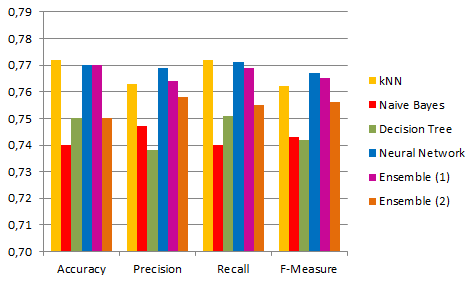
\includegraphics[width=\columnwidth]{../../charts/results.png}
	\caption{Evaluation metrics of the different classifiers}
	\label{fig:result}
\end{figure}

\begin{figure}[H]
	\centering
	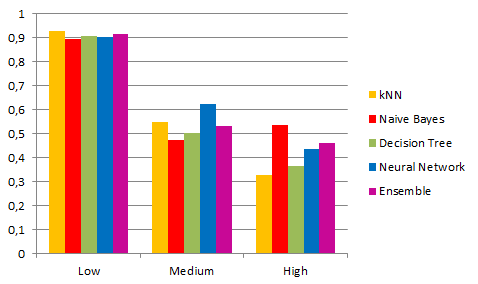
\includegraphics[width=\columnwidth]{../../charts/recall.png}
	\caption{Recall of the different classifiers}
	\label{fig:recall}
\end{figure}

\subsection{Discussion}

Considering all the evaluation metrics shown in \fref{fig:result}, the Neural Network delivered the best results in every case. Contrary to the initial believe that the majority voting would enhance the results, it turned out that they were merely average. 
 
To compare our results with those of \cite{indian}, it should be considered that on the one hand they used predefined ranges for their classification and on the other hand they used different attributes, mostly focusing on income and education.



